%%%%%
%%Title: HiPi+Bus V0.1 Chapter 4 Section 5
%%Creator: Ando Ki
%%CreationDate: April 1992
%%FileName: sec5
%%RelatedFile: ch4
%%%%%
\section{인터럽트 버스 중재}
인터럽트 버스 중재(interrupt bus arbitration)는 인터럽트의 전송을 원하는
인터럽트 요청기들이 동시에 여러개가 존재할
수 있기 때문에 이를 충돌없이 처리하기 위해 필요한 동작이다. 
따라서 인터럽트 버스 상의 인터럽트 전송은 항상 요청기에 의한 중재 주기부터 시작된다.
인터럽트 요청기는 진행 중인 인터럽트의 마지막 단계에서 IBSYNC* 구동을 멈춤으로써
다음 주기가 중재 주기가 될 수 있음을 알린다.
이때 인터럽트를 보낼 요청기가 있으면 중재 주기가 시작되고,
중재 방법은 8 비트의 부호화된 자가 중재 기법(coded self arbitration scheme)을 사용한다.
중재 주기에서 우선 순위 경쟁을 위하여 사용하는 정보는 인터럽트 종류(interrupt class),
요청기의 구별자(id address)이며 항상 우선 순위 방법을 사용한다.
중재에서는 패리티를 사용하지 않는다.
인터럽트 중재 주기는 5개 버스 클럭 주기동안 수행된다. \\
%
\subsection{중재 정보}
중재 주기에서 각 요청기가 사용하는 중재 정보는 {\tt <}표~\ref{table:int-arb}{\tt >}와 같다.
%\documentstyle[a4]{hbook}
%\begin{document}
%
\begin{table}[htbp]
\caption{인터럽트 버스 중재에 사용되는 중재 정보}\label{table:int-arb}
   \begin{center}
   \begin{tabular}{|l|l|} \hline
	bit field & information \\
\hline \hline
	7, 6       & interrupt class \\ \hline
	5, 4, 3, 2 & ida$<$5..2$>$ \\ \hline
	1, 0       & ida$<$1..0$>$ \\ \hline
   \end{tabular}
   \end{center}
\end{table}
%
%\end{document}

비트 7부터 비트 0가 IBD{\tt <}7..0{\tt >}*의 신호에 각각 대응되어 구동되고,
중재 주기에서는 패리티 비트는 사용하지 않는다.
비트 0부터 5까지는 {\tt <}표~\ref{table:int-ga}{\tt >}에
나타낸 요청기 구별자가 되고,
비트6, 7은 {\tt <}표~\ref{table:int-class}{\tt >}에 나타낸 인터럽트의 종류을 나타내는데, 
그 숫자가 클수록 중재에 있어서 높은 우선 순위를 갖는다.
비트 6, 7은 인터럽트의 종류에 따른 우선 순위 정보이외에
인터럽트 요청의 존재 유무(0일 경우 No interrupt)를 나타낸다. \\
{\tt <}표~\ref{table:int-arb}{\tt >}의 비트 0부터 5까지는 요청기 구별자를 나타내는데,
요청기 구별자는 {\tt <}표~\ref{table:int-ga}{\tt >}과 같다.
%\documentstyle[a4]{hbook}
%\begin{document}
%
\begin{table}[htbp]
\caption{인터럽트 중재 주기에 사용되는 구별자 배정}\label{table:int-ga}
   \begin{center}
   \begin{tabular}{|c|l|l|}
\hline
Slot ID & \multicolumn{2}{|c|}{Interrupt Requester Identification Address} \\ \cline{2-3}
	        & ida$<$5..2$>$ & ida$<$1..0$>$ \\
\hline \hline
	 0 - 9  & GA$<$3..0$>$ & {\it reserved\/} \\ \hline
	10      & GA$<$3..0$>$ & {\it reserved\/} \\
	        & 0x15                 & {\it reserved\/} \\ \hline
	11 - 12 & GA$<$3..0$>$ & {\it reserved\/} \\ \hline
	13 - 20 & \multicolumn{2}{|c|}{{\it undefined\/}} \\
\hline
   \end{tabular}
   \end{center}
\end{table}
%
%\end{document}

요청기가 위치하는 슬롯 어드레스에 따라 요청기 구별자(ida{\tt <}5..0{\tt >})가
결정되는데 슬롯0에서 12 까지는 4개씩의 요청기가 배정될 수 있고,
슬롯13 부터 슬롯20 까지는 정의를 유보한다.
슬롯10은 시스템 콘트롤러가 삽입되는 곳으로 요청기 구별자가 4 개 더 배정된다.
슬록10번의 경우 시스템 제어에 관련된 인터럽트를 수행할 경우는 
가장 높은 우선 순위를 사용하고, 일반적인 입출력 동작을 할 경우는 자신의 보통의 요청기 구별자를
사용할 수 있도록 하기 위함이다.
%
\subsection{부호화된 자가 중재 기법}
부호화된 자가 중재 기법(coded self arbitration scheme : CSAS)은
wired-OR 버스의 특성을 이용한 중재 방법으로
버스를 요청하는 모든 모듈에 중재기(distributed arbiter)를 갖고, 
각 중재기에 고유의 번호(인터럽트 버스에서는 슬롯 어드레스)를 코드화하여 할당한다.
버스는 wired-OR 특성을 갖기 때문에  동시에 여러 모듈이 버스에 신호를 구동하였을 경우
low 값만 나타나게 된다. 중재가 진행되는 방법은, 버스 모듈들은 동시에 중재정보(중재번호)를
구동하고 모든 신호가 버스 상에서 안정된 후 자신이 구동한 중재번호가 버스에 나타나면 중재에서 이긴것이고,
그러하지 않을 경우 신호의 구동을 멈추고 다음 중재 주기까지 기다리게 된다.
CSAS 방법을 사용하려면 버스의 신호선은 중재를 원하는 모듈 수에
$\log_{2}$를 취한 수\footnote{$n = \lceil \log_{2} N \rceil$ ; n은 필요한 버스의 신호선 수,
N은 모듈의 수; $\lceil x \rceil$ denotes the least integer that is
greater than or equal to x.}
만큼이 필요하고, wired-OR 기능이 있는 신호선을 사용해야 하며,
중재 시간은 신호의 수에 비례하게 된다.
{\tt <}그림~\ref{figure:csa}{\tt >}는 CSAS을 이용한 중재기의
일례이다.
%
\begin{figure}[hp]
    \centerline{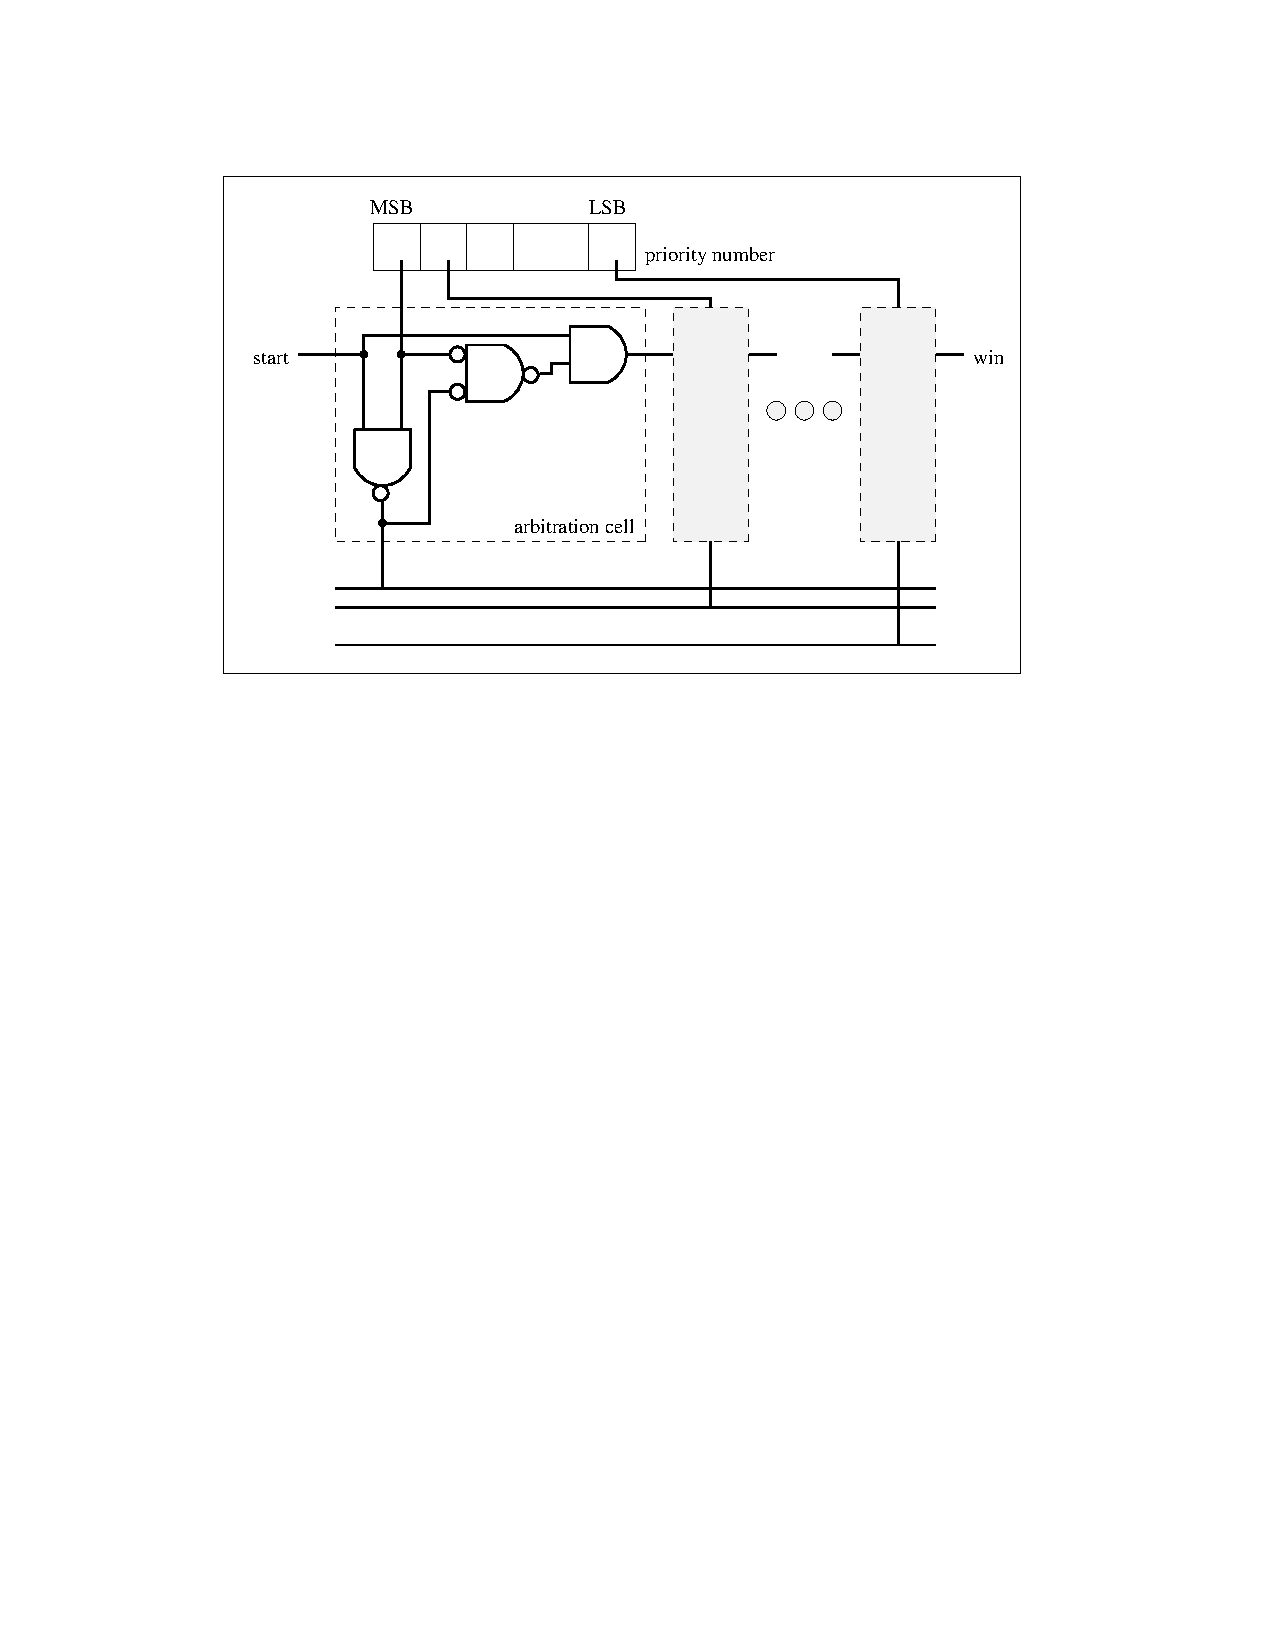
\includegraphics{ch4/FIG/int-arbiter.jpg}}
   \caption{부호화된 자가 중재기의 일례}\label{figure:csa}
\end{figure}
%
%
